
\section{Exercises}

\begin{excersizelist}

\item \label{exer:multiplieropampwithmodel}  Analyse the inverting amplifier circuit in Figure~\ref{circ:opampinvertingamplifierequivalent} to obtain the relationship between input voltage $x$ and output voltage $y$ given by~\eqref{eq:intertingopampmodel}.  You may wish to use a symbolic programming language (for example Maxima, Sage, Mathematica, or Maple).
\begin{solution}
We provide two solutions.  Let $v_i$, $v_o$, $v_1$ and $v_2$ be the voltages over the input resistor $R_i$, the output resistor $R_o$, and resistors $R_1$ and $R_2$ respectively.  Observe that $v_+ - v_i = v_i$ and so the voltage over the dependent source is $A v_i$.  The voltages satisfy,
\begin{align*}
x &= v_1 - v_i \\
y &= -v_i - v_2 \\
y &=  v_o + Av_i
\end{align*}
The currents into the 3 way connection between $R_i, R_1$ and $R_2$ sum to zero, and so
\[
\frac{v_1}{R_1} + \frac{v_i}{R_i} = \frac{v_2}{R_2}
\]
by Ohm's law, the direction of current moving from positive to negative voltage.  Finally the currents through $R_o$ and $R_2$ are the same, and so
\[
\frac{v_o}{R_o} = \frac{v_2}{R_2}.
\]
We now have 5 linearly independent equations for the six unknowns $v_1, v_2, v_o, v_i, x, y$.  We can use these to find an equation that describes $y$ in terms of $x$.  The Mathematica command
\begin{verbatim}
Simplify[Solve[{x == v1 - vi,
   y == vo + A*vi,
   y == -vi - v2,
   v1/r1 + vi/ri == v2/r2,
   vo/ro == v2/r2,
   r1 > 0, r2 > 0, ro > 0, ri > 0, A > 0},
  {y, vi, vo, v2, v1}, Reals]]
\end{verbatim}
or Maxima command
\begin{verbatim}
linsolve([x = v1 - vi,
   y = vo + A*vi,
   y = -vi - v2,
   v1/r1 + vi/ri = v2/r2,
   vo/ro = v2/r2],
   [y, vi, vo, v2, v1]);
\end{verbatim}
readily obtains
\[
y = \frac{R_i (R_o - A R_2) }{R_i (R_2+R_o)+R_1 (R_2+R_i + A R_i+R_o)}x.
\]

The second solution is thanks to Badri Vellambi.  Consider the operational amplifier circuit with feedback presented in Fig.~\ref{Fig-Prob2.1a}. Suppose that the voltage signal fed into the circuit is $x(t)$ and the voltage signal measured at the output of the opamp is $y(t)$. 

{
\centering
\captionsetup{type=figure}
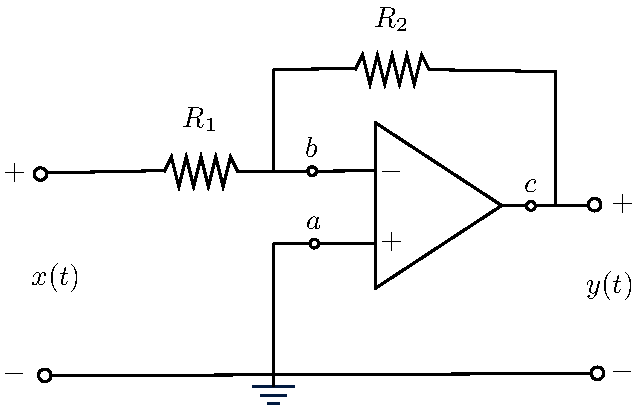
\includegraphics[width=3in]{plots/multiplierbadri1.pdf}
\captionof{figure}{The circuit}
 \label{Fig-Prob2.1a}
}

To simplify the circuit, one has to use the model for the opamp given in Fig.~\ref{Fig-Prob2.1b} which involves the voltage-controlled voltage-source (VCVS) at the output side (indicated in green).  While replacing the operational amplifier with its model, it must be noted that the positive terminal of the operational amplifier is connected to the ground.

{
\centering 
\captionsetup{type=figure}
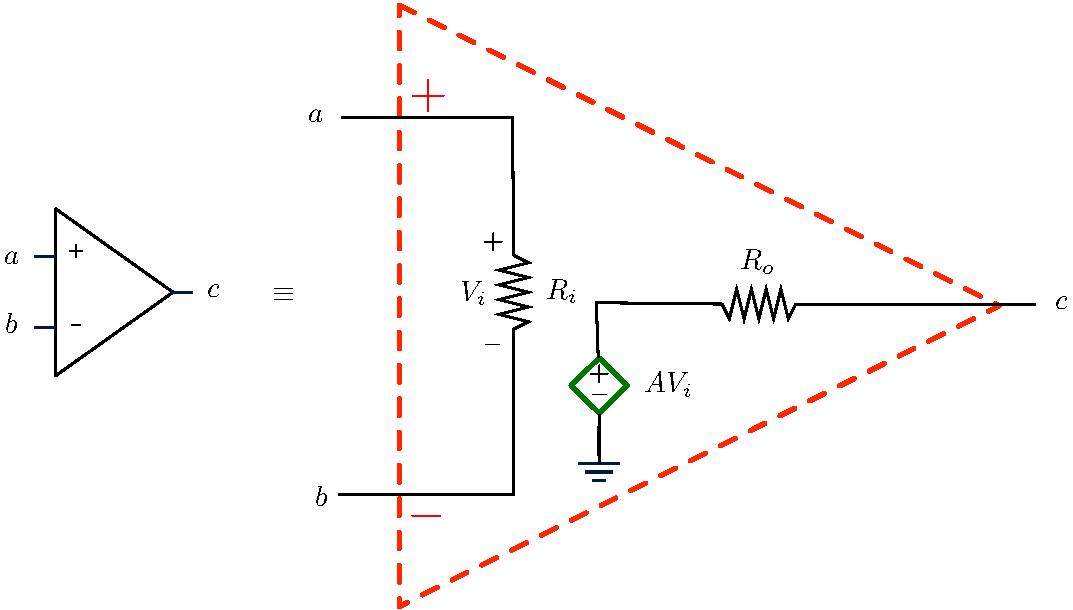
\includegraphics[width=5in]{plots/multiplierbadri2.pdf}
\captionof{figure}{The model for an operational amplifier}
 \label{Fig-Prob2.1b}
}

Upon replacement, we obtain the following equivalent circuit. Again notice that since the positive terminal of the opamp was connected to the ground, the voltage output by the VCVS is $AV_i$ where $V_i$ is the voltage between the ground and the top of the resistance $R_i$, and is measured against the flow of the current $i-i_1$ as is indicated in the figure.

{
\centering 
\captionsetup{type=figure}
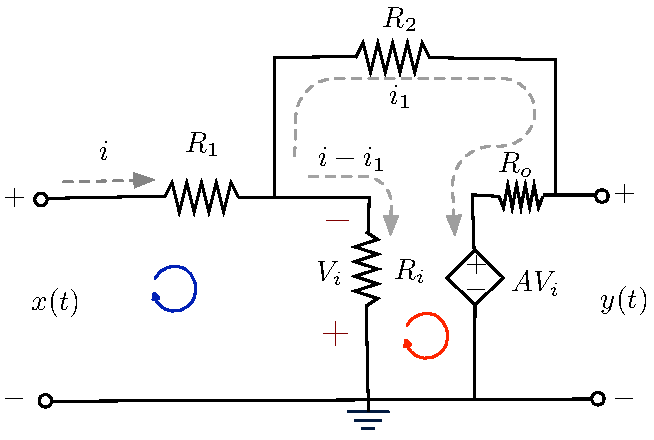
\includegraphics[width=4in]{plots/multiplierbadri3.pdf}
\captionof{figure}{The operational amplifier circuit with the model}
 \label{Fig-Prob2.1c}
}

Applying Kirchoff's law to the outer loop indicated in blue in Fig.~\ref{Fig-Prob2.1c}, we obtain the following equation.
\begin{equation}
x(t) = iR_1+(i-i_1)R_i = i(R_1+R_i) - i_1 R \label{eqn-Prob2.1.1}
\end{equation}
Note that by definition, the voltage $V_i$ that controls the VCVS is the voltage across $R_i$ measured against the indicated direction of the current $i-i_1$, and is given by
\begin{equation}
V_i = -(i-i_1)R_i. \label{eqn-Prob2.1.2}
\end{equation}
Next, writing out the Kirchoff's law for the inner loop indicated in red, we obtain the following.
\begin{align}
0 &= i_1 R_2 + i_2 R_0 + AV_i - (i-i_1) R_i
\end{align}
Substituting $V_i$ in the above equation with the RHS of \eqref{eqn-Prob2.1.2}, we obtain the following.
\begin{align}
0&= i_1 (R_2+R_0) - A(i-i_1)R_i-(i-i_1)R_i\\
&= -i(1+A)R_i+i_1((1+A)R_i+R_0+R_2)\label{eqn-Prob2.1.3}
\end{align}
Combining \eqref{eqn-Prob2.1.3} and \eqref{eqn-Prob2.1.1}, we obtain the following linear system of equations governing the electrical circuit.
\begin{align}
\left[\begin{array}{cc} R_1+R_i &  -R_i\\ -(1+A)R_i & (1+A)R_i+R_0+R_2\end{array}\right]\left[\begin{array}{c} i\\ i_1\end{array}\right] = \left[\begin{array}{c} x(t)\\ 0\end{array}\right]
\end{align}
Solving the above linear system, we identify the current in the different branches to be
\begin{align}
\left[\begin{array}{c} i\\ i_1\end{array}\right] = x(t)\left[\begin{array}{c} \frac{ (1+A)R_i+R_0+R_2}{(1+A) R_iR_1+R_0R_1+R_2R_1+R_0R_i+R_2R_i}\\ \frac{(1+A)R_i}{(1+A) R_iR_1+R_0R_1+R_2R_1+R_0R_i+R_2R_i}\end{array}\right].\label{eqn-Prob2.1.4}
\end{align}
Lastly, notice that
\begin{align}
y(t) &= i_1 R_0 + A V_i \\
 & = i_1 R_0 - (i-i_1)R_i.
\end{align}
Substituting the solutions for $i$ and $i_1$ in terms of $x(t)$, we obtain the following.
\begin{align}
y(t)= \left( \frac{R_iR_0 - R_2R_iA}{(1+A) R_iR_1+R_0R_1+R_2R_1+R_0R_i+R_2R_i} \right)x(t)
\end{align}


\end{solution}

\end{excersizelist}


%%% Local Variables: 
%%% mode: latex
%%% TeX-master: "main.tex"
%%% End: 
